% Turabian Formatting for Research Papers Template, 2018/08/06
%
% Developed using the turabian-formatting package (2018/08/01), available through CTAN: http://www.ctan.org/pkg/turabian-formatting
%
% Additional document class formatting options:
%
% raggedright: ragged right formatting without hyphenations
% authordate: support for the author-date citation style
% endnotes: support for endnotes



\documentclass[12pt]{turabian-researchpaper}


\usepackage[utf8]{inputenc}
\usepackage{csquotes, ellipsis,xurl,tocloft,graphicx}

% Specify paper size with geometry package
\usepackage[pass, letterpaper]{geometry}

% For citations, use the biblatex-chicago package
\usepackage{biblatex-chicago}
\addbibresource{works-cited.bib}

% Numbering the sections
\setcounter{secnumdepth}{2}
\setcounter{tocdepth}{2}
\renewcommand{\cftsecleader}{\cftdotfill{\cftdotsep}}

% Information for title page
\title{TEMP TITLE}
\subtitle{TEMP SUBTITLE}
\author{Eric Altenburg}
\course{HST 415: The Nuclear Era}
\date{\today}

\raggedright


\begin{document}

\maketitle

Coming off the heels of World War II when Eastern Europe and parts of the world were trying to recover, there was a difference in ideologies forming. The nations that were being helped by the United States adopted capitalism, whereas those under the Soviet Union employed the communist methodology. Capitalism versus communism is what initiated the Cold War with the United States and the Soviet Union being the two leading actors. Shortly thereafter, the Soviet Union developed and successfully tested their own nuclear weapons giving way to a new threat in the eyes of the United States; there was now another nuclear superpower. Knowing that the United States was no longer in nuclear control led to a growing anxiety among its citizens with fears of a nuclear war coming to cities where millions lived. Further adding to this stress was a film called "Duck and Cover" released by the Civil Defense Firm which depicted what to do in the event of a nuclear explosion. With the nation on edge in fear of a nuclear war breaking out, tensions rose once more with the Red Scare and McCarthyism—a movement to oust communists in the United States through accusations without a proper regard for any evidence. Therefore, with the nation whose stress levels were at an all time high, the only thing that gave them a sense of well-being and safety were fallout shelters. These locations were marked with an iconic yellow and black sign, and they were meant to provide safety for occupants from radioactive debris and fallout from a nuclear blast. However, creating these places on such short notice was difficult and expensive, so a solution was to inspect all known buildings to see if they met the requirements of a fallout shelter. But it was often the case that these buildings were constructed too long ago to adequately hold up against a nuclear blast—not that any buildings were realistically capable of withstanding such a blast—and because of this, Americans were encouraged to build their own in their backyard. This idea of having people find their own solutions causes problems, specifically this creates an issues of selectively choosing who can and cannot survive a nuclear war. While not necessarily inherently racist or biased towards one race, the distribution of the shelters was centered around areas that were found to be newer and able to withstand a blast, and they were often found in areas where the surrounding population was wealthier and had more money flowing through. Additionally, since families were encouraged to build their own bunkers and fallout shelters in the event of a nuclear explosion, this meant they were expected to be able handle the enormous upfront cost to build such a structure. Not all families in the United States had the means and extra income to afford a project like that. This preference toward wealthy families coupled with the wage gap between races in the years of the Cold War shows that while not explicitly targeting white communities to build fallout shelters, they were indirectly prioritized. 





% \begin{figure}[!h]
%     \centering
%     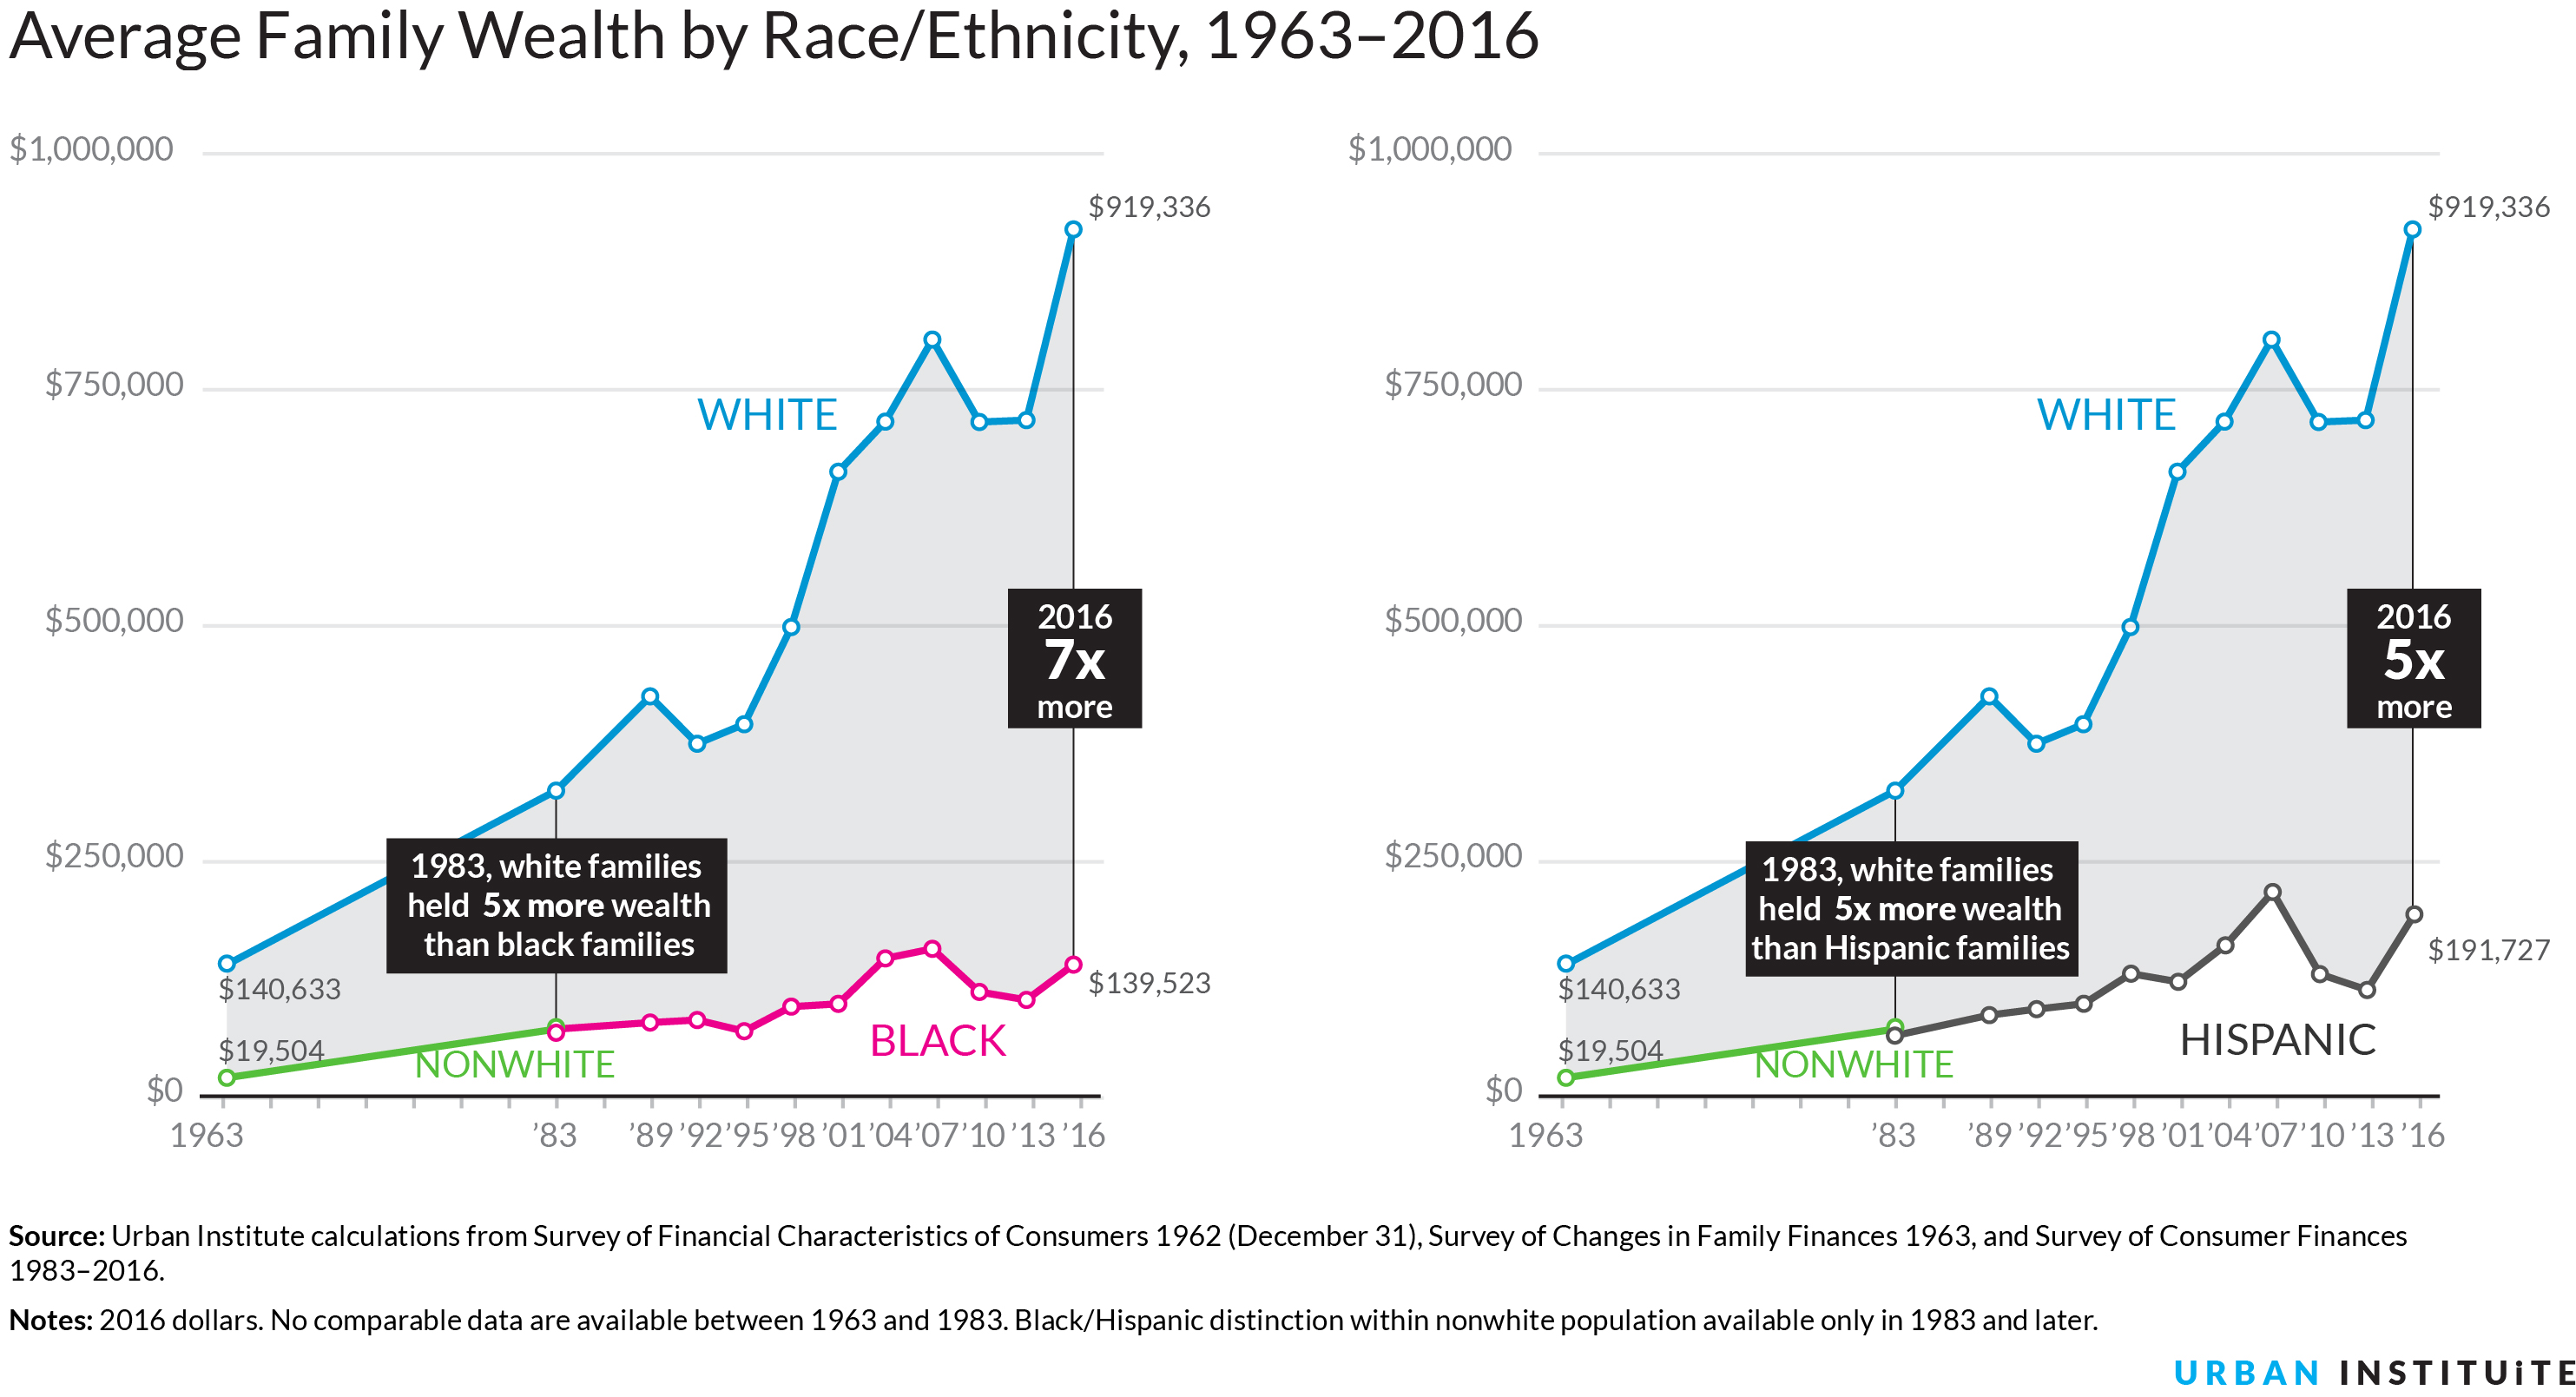
\includegraphics[scale=0.6]{images/WealthByRace-avg.jpeg}
%     \caption{This shows the disparity between the average wages of white and nonwhite families.}
%     \label{WealthAvg}
% \end{figure}



\newpage
\begin{thebibliography}{100}
	% \bibitem{1}{Lewis, Jeffrey. 2018. \textit{The 2020 Commission Report on the North Korean Nuclear Attacks Against the United States}. Houghton Mifflin Harcourt.}
\end{thebibliography}

\end{document}